\documentclass[11pt, a4paper]{article}
\usepackage[utf8]{inputenc}
\usepackage{geometry}
\geometry{margin=1in}
\usepackage{graphicx}
\usepackage{bookmark}
\usepackage{hyperref}
\usepackage{tikz}
\usetikzlibrary{shapes, arrows.meta, positioning, fit, backgrounds}
\usepackage{titlesec}
\usepackage{lipsum}

% Title Component
\title{\textbf{Assignment 4: Sri Tel - New Customer Experience}\\ \large Service Oriented Computing (CSS4242/CSC4222)}
\author{Group Members:\\ H.S.R. Yasas (SC/2020/11431) \\ T.G.M.M.Ferdinandaz (SC/2020/11446)}
\date{}

\begin{document}

\maketitle
\tableofcontents
\newpage

\section{Introduction}
Sri Tel Ltd (STL), a telecommunication provider offering GSM/3G/4G/LTE services, aims to increase market share by improving customer care and experience. The current initiative involves deploying a state-of-the-art "Sri-Care" solution comprising a web portal and smartphone applications (iOS/Android).

The primary objective of this solution is to allow existing customers to manage their accounts, pay bills, and activate services without manual intervention from support staff. The solution must integrate with an existing Provisioning System and an external Payment Gateway while ensuring scalability, security, and high availability for notification delivery.

\section{Proposed Architectures}
To address the requirements of scalability, multi-client support (Web \& Mobile), and integration with external systems, we analyzed two distinct architectural approaches.

\subsection{Alternative Architecture 1: Service-Oriented Architecture (SOA) with ESB}
The first approach utilizes a traditional Service-Oriented Architecture centered around an Enterprise Service Bus (ESB).

\textbf{Description:}
In this model, an ESB acts as the central backbone. All client requests are routed through the ESB, which orchestrates calls to various backend services. The ESB handles message transformation, protocol bridging, and routing.

\begin{figure}[h]
\centering
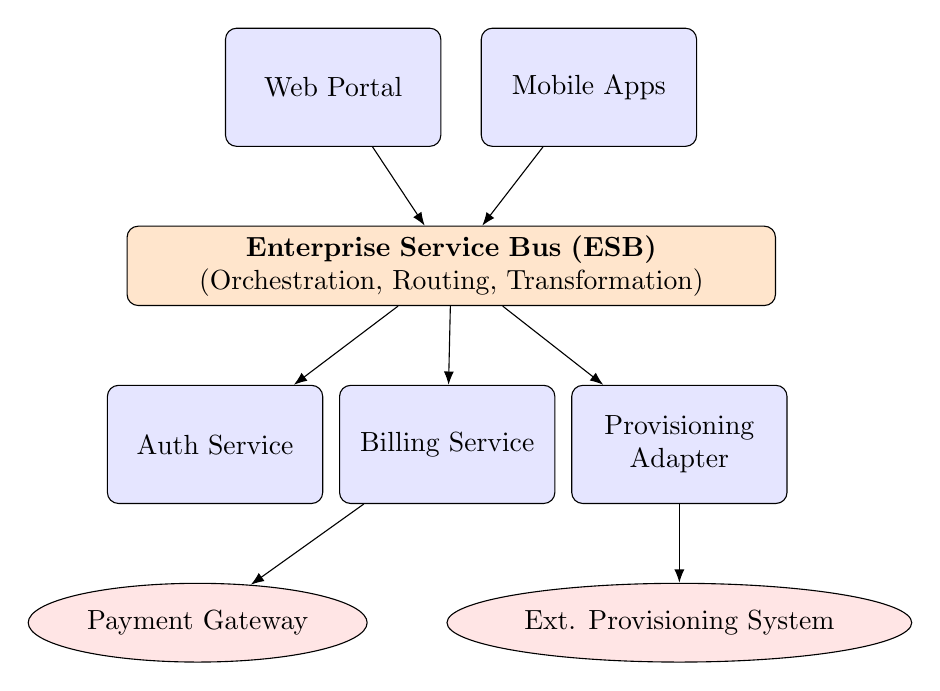
\begin{tikzpicture}[node distance=2cm, auto,
    block/.style={rectangle, draw, fill=blue!10, text width=2.5cm, text centered, rounded corners, minimum height=1.5cm},
    esb/.style={rectangle, draw, fill=orange!20, text width=8cm, minimum height=1cm, text centered, rounded corners},
    cloud/.style={draw, ellipse, fill=red!10, node distance=3cm, minimum height=1cm},
    line/.style={draw, -Latex}
]
    % Clients
    \node [block] (web) {Web Portal};
    \node [block, right=0.5cm of web] (mobile) {Mobile Apps};
    
    % ESB
    \node [esb, below=1cm of web, xshift=1.5cm] (esb) {\textbf{Enterprise Service Bus (ESB)} \\ (Orchestration, Routing, Transformation)};
    
    % Services
    \node [block, below=1cm of esb, xshift=-3cm] (auth) {Auth Service};
    \node [block, right=0.2cm of auth] (billing) {Billing Service};
    \node [block, right=0.2cm of billing] (prov) {Provisioning Adapter};
    
    % External
    \node [cloud, below=1cm of prov] (ext_prov) {Ext. Provisioning System};
    \node [cloud, left=1cm of ext_prov] (ext_pay) {Payment Gateway};

    % Connections
    \path [line] (web) -- (esb);
    \path [line] (mobile) -- (esb);
    \path [line] (esb) -- (auth);
    \path [line] (esb) -- (billing);
    \path [line] (esb) -- (prov);
    \path [line] (prov) -- (ext_prov);
    \path [line] (billing) -- (ext_pay);
\end{tikzpicture}
\caption{Alternative 1: SOA with ESB}
\end{figure}

\textbf{Pros and Cons:}
\begin{itemize}
    \item \textbf{Pros:} Strong integration capabilities; centralized management of policies; mature technology for protocol mediation.
    \item \textbf{Cons:} The ESB can become a single point of failure and a performance bottleneck; logic often bleeds into the ESB (smart pipes), making it harder to scale individual components; heavy-weight for simple mobile app backends.
\end{itemize}

\subsection{Alternative Architecture 2: Microservices Architecture (Selected)}
The second and selected approach is a Microservices Architecture utilizing an API Gateway and Event-Driven asynchronous communication for notifications.

\textbf{Description:}
The application is broken down into small, independent services (User, Bill, Notification, Provisioning). An API Gateway sits in front of the services, handling routing, authentication, and rate limiting. Inter-service communication is primarily RESTful for synchronous operations and Message-based (Pub/Sub) for asynchronous tasks like notifications.

\begin{figure}[h]
\centering
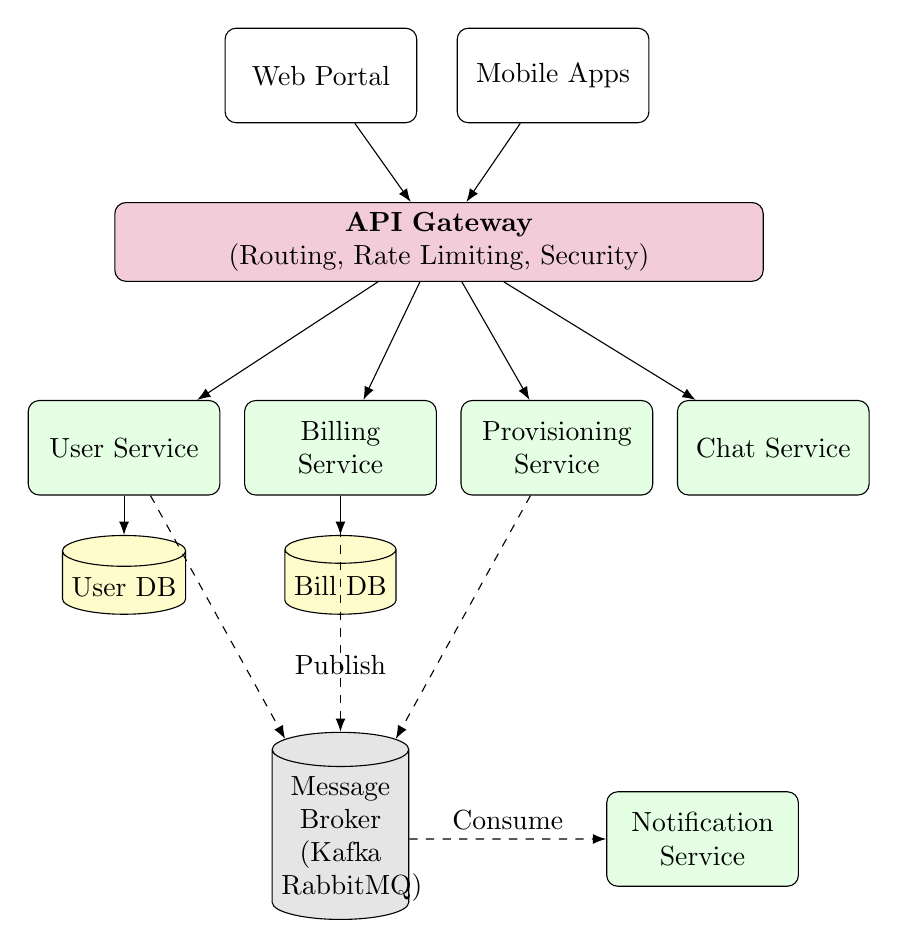
\begin{tikzpicture}[node distance=1.5cm, auto,
    service/.style={rectangle, draw, fill=green!10, text width=2.2cm, text centered, rounded corners, minimum height=1.2cm},
    gateway/.style={rectangle, draw, fill=purple!20, text width=8cm, minimum height=1cm, text centered, rounded corners},
    queue/.style={cylinder, shape border rotate=90, draw, fill=gray!20, aspect=0.25, text width=1.5cm, text centered},
    db/.style={cylinder, shape border rotate=90, draw, fill=yellow!20, aspect=0.25, minimum height=1cm},
    line/.style={draw, -Latex}
]

    % Clients
    \node [service, fill=white] (web) {Web Portal};
    \node [service, fill=white, right=0.5cm of web] (mobile) {Mobile Apps};
    
    % Gateway
    \node [gateway, below=1cm of web, xshift=1.5cm] (gw) {\textbf{API Gateway} \\ (Routing, Rate Limiting, Security)};
    
    % Services
    \node [service, below=1.5cm of gw, xshift=-4cm] (user) {User Service};
    \node [service, right=0.3cm of user] (bill) {Billing Service};
    \node [service, right=0.3cm of bill] (prov) {Provisioning Service};
    \node [service, right=0.3cm of prov] (chat) {Chat Service};
    
    % Message Broker and Notification
    \node [queue, below=3cm of bill] (broker) {Message Broker (Kafka\\RabbitMQ)};
    \node [service, right=2.5cm of broker] (notif) {Notification Service};
    
    % DBs
    \node [db, below=0.5cm of user] (db1) {User DB};
    \node [db, below=0.5cm of bill] (db2) {Bill DB};

    % Connections
    \path [line] (web) -- (gw);
    \path [line] (mobile) -- (gw);
    \path [line] (gw) -- (user);
    \path [line] (gw) -- (bill);
    \path [line] (gw) -- (prov);
    \path [line] (gw) -- (chat);
    
    \path [line, dashed] (bill) -- (broker) node[pos=0.8, above] {Publish};
    \path [line, dashed] (prov) -- (broker);
    \path [line, dashed] (user) -- (broker);
    \path [line, dashed] (broker) -- (notif) node[midway, above] {Consume};
    
    \path [line] (user) -- (db1);
    \path [line] (bill) -- (db2);
\end{tikzpicture}
\caption{Selected Architecture: Microservices with Event-Driven Notifications}
\end{figure}

\subsection{Rationale for Selection}
We selected the \textbf{Microservices Architecture} for the Sri-Care solution for the following reasons:
\begin{itemize}
    \item \textbf{Scalability:} The notification service is expected to handle high volumes ("best effort"). Microservices allow us to scale the Notification Service and Message Broker independently of the User or Billing services.
    \item \textbf{Agility:} The "Sri-Care" portal and apps require frequent updates. Independent deployment of microservices allows faster iteration without redeploying the entire monolith.
    \item \textbf{Technology Heterogeneity:} We can use Node.js for the I/O-bound Chat service and Java/Spring Boot for the transaction-heavy Billing service.
    \item \textbf{Fault Isolation:} A failure in the Chat service will not impact the critical Billing or Provisioning functionalities.
\end{itemize}

\section{Architectural and Integration Patterns}
Referencing the course notes on Microservices and Integration Patterns, the following patterns are implemented:

\subsection{Architectural Patterns}
\begin{itemize}
    \item \textbf{API Gateway Pattern:}
    Single entry point for all clients (Web and Mobile). It abstracts the underlying microservices, aggregates responses (reducing round trips for mobile users), and enforces security policies (SSL termination, Authentication).
    
    \item \textbf{Database per Service:}
    Each microservice (User, Billing) owns its database schema to ensure loose coupling. Changes to the Billing database do not impact the User service.
    
    \item \textbf{Backend for Frontend (BFF):}
    Although a single Gateway is proposed, logically we treat the APIs as catering to specific needs of the mobile/web clients, allowing optimized data payloads.
\end{itemize}

\subsection{Integration Patterns}
\begin{itemize}
    \item \textbf{Publish-Subscribe Channel (Messaging):}
    Used for the Notification requirement. When a bill is generated or a service activated, the Billing Service publishes an event to the Message Broker (e.g., RabbitMQ). The Notification Service subscribes to this channel. This ensures the "best effort" delivery and prevents the main user flow from blocking while waiting for email/SMS sending.
    
    \item \textbf{Adapter Pattern:}
    The solution includes a "Provisioning Adapter" (or Anti-Corruption Layer) that translates internal REST domain calls into the specific format required by the external Telco Provisioning System.
\end{itemize}

\section{Information Security Considerations}
\begin{itemize}
    \item \textbf{Authentication \& Authorization (OAuth 2.0 / OIDC):}
    Using an Identity Provider (IdP) like Keycloak. The Mobile App and Web Portal authenticate against the IdP and receive an Access Token (JWT). The API Gateway validates this token before forwarding requests.
    \item \textbf{Transport Security (TLS/HTTPS):}
    All communication between clients and the Gateway, and between internal services, is encrypted.
    \item \textbf{Network Isolation:}
    The Microservices and Databases reside in a private subnet, not directly accessible from the internet. Only the API Gateway and Load Balancer are exposed publicly.
    \item \textbf{Secure Configuration:}
    Secrets (DB passwords, API keys for Payment Gateway) are managed via a Vault or Config Server, not hardcoded.
\end{itemize}

\section{Chat Module Architecture}
Although the chat implementation is optional, the architecture supports it via \textbf{WebSockets}.
\begin{itemize}
    \item The Chat Service is a dedicated microservice keeping persistent WebSocket connections with the User App and the Agent Console.
    \item It uses a lightweight, event-driven runtime (e.g., Node.js or Go) to handle thousands of concurrent open connections.
    \item Redis is used as a Pub/Sub mechanism for syncing messages if the Chat Service is scaled horizontally across multiple instances.
\end{itemize}

\section{Conclusion}
The proposed Microservices solution effectively addresses Sri Tel's needs for a modern, scalable customer care platform. By leveraging the API Gateway for unified access and an Event-Driven architecture for high-volume notifications, the system ensures robustness and a superior user experience.

\end{document}
